\chapter{Detailed design}

In this chapter, every single class is described in terms of public interface
and functionality. Because of the fairly dynamic character of this project --
new ideas come and go -- this chapter will not be finished until the end of the
project and will probably change regularly.

\section{Files and directories}

All source code will be in the directory \texttt{src/}. All classes are in the
package \texttt{amber} or in a subpackage thereof. The Psyclone specification
file \texttt{psySpec.xml} is found in \texttt{data/}. External libraries that
are redistributed with \Amber\ are in \texttt{lib/}. The source of this
document, the traineeship report and the website are located in
\texttt{documentation/}.

The application is built using Apache
Ant\footnote{\url{http://ant.apache.org/}} and it can be imported into
Eclipse\footnote{\url{http://www.eclipse.org/}}. It requires Java SDK version
1.5 or greater.

\section{Classes}

\begin{figure}[htp]
  \centering
  \includegraphics{image/class-diagram-launcher}
  \caption{The inheritance model of the Launcher class}
  \label{fig:class-diagram-launcher}
\end{figure}

\begin{figure}[p]
  \centering
  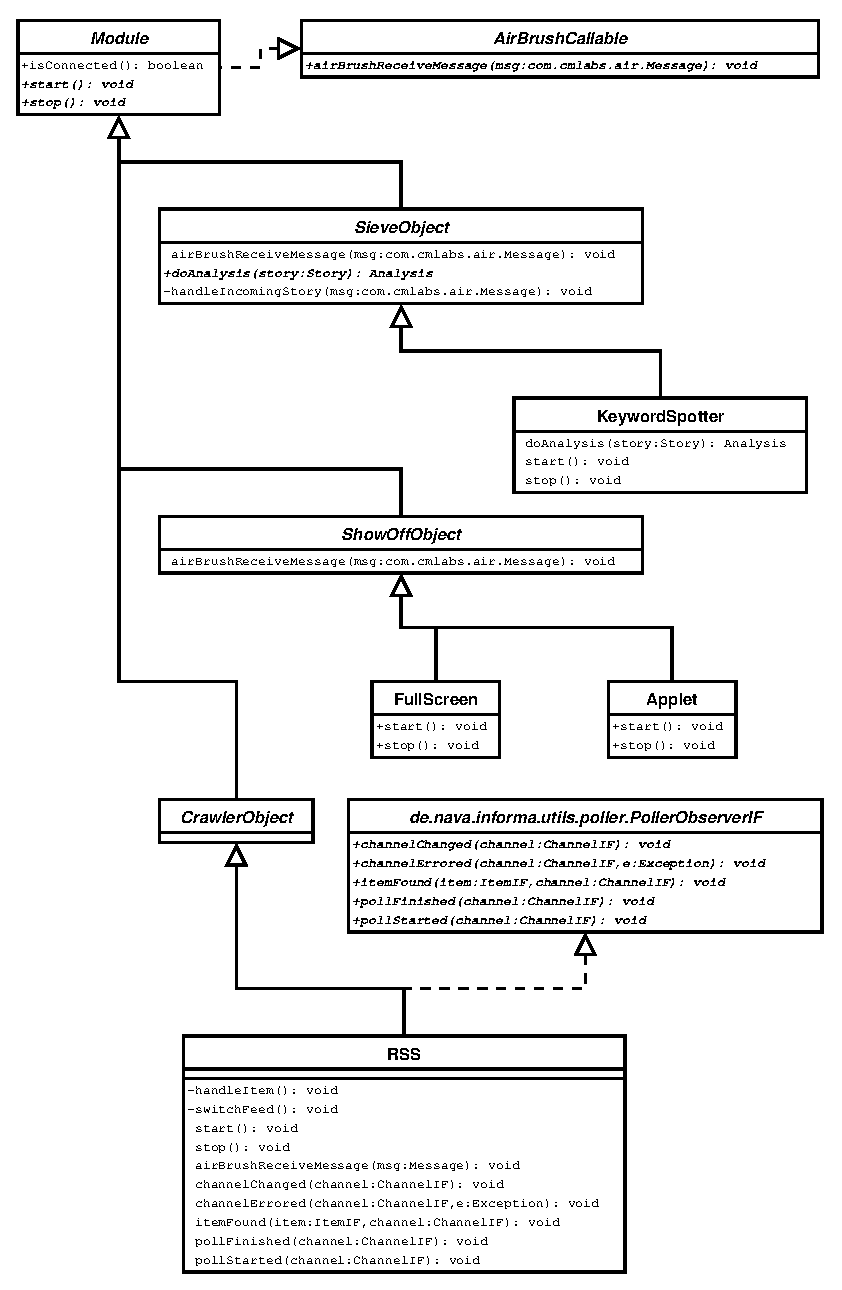
\includegraphics{image/class-diagram-module}
  \caption{The inheritance model of the Module class}
  \label{fig:class-diagram-launcher}
\end{figure}

\begin{figure}[p]
  \centering
  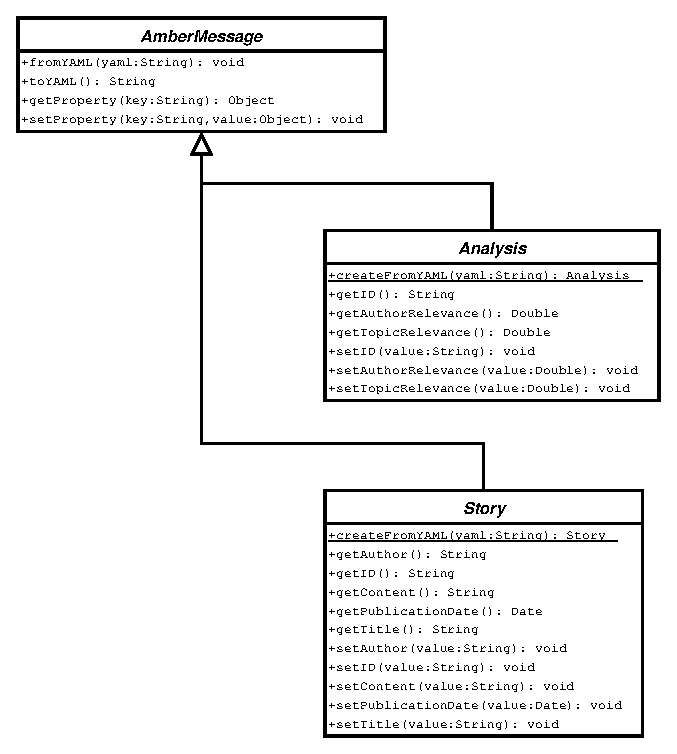
\includegraphics{image/class-diagram-ambermessage}
  \caption{The inheritance model of the AmberMessage class}
  \label{fig:class-diagram-launcher}
\end{figure}

\begin{figure}[p]
  \centering
  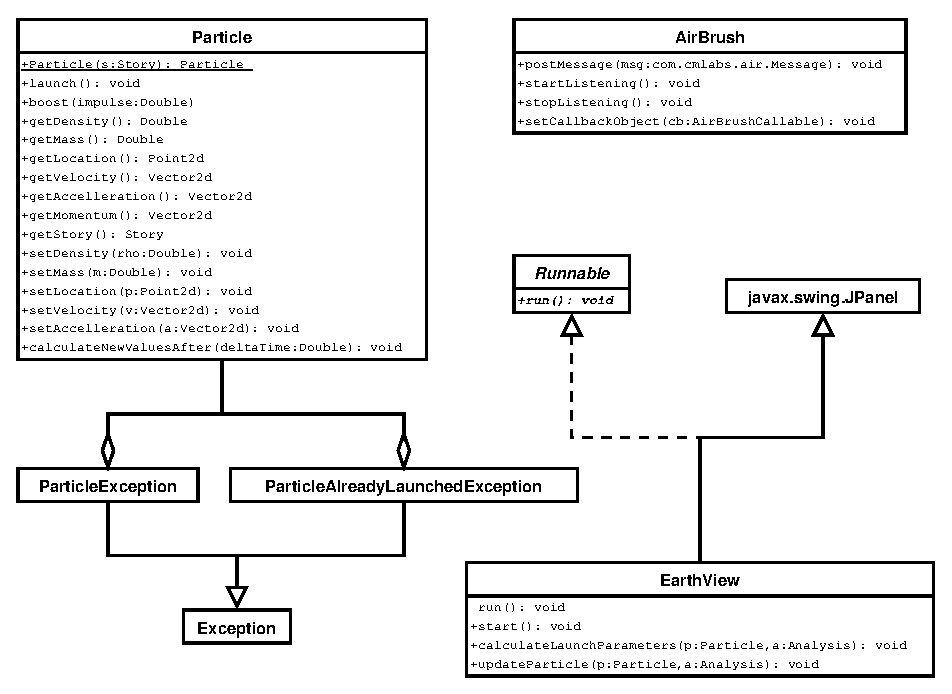
\includegraphics{image/class-diagram}
  \caption{The inheritance model of the remaining classes}
  \label{fig:class-diagram-launcher}
\end{figure}


\section{Objects in the amber package}

The classes in the main package are launchers for the three different modules
and abstract classes for the main objects of these modules. Basically it works
like this; if the Crawler class is started it creates a CrawlerObject and
starts it.

\classname{Crawler}

\begin{classmetadata}
\end{classmetadata}

\begin{interface}
\end{interface}



\classname{CrawlerObject}

\begin{classmetadata}
\end{classmetadata}

\begin{interface}
\end{interface}



\classname{ShowOff}

\begin{classmetadata}
\end{classmetadata}

\begin{interface}
\end{interface}



\classname{ShowOffObject}

\begin{classmetadata}
\end{classmetadata}

\begin{interface}
  \method{\void}{start}{}
    {Starts the ShowOff module.}
  \method{\void}{stop}{}
    {Stops the ShowOff module.}
  \method{\void}{setStoryQueue}{Queue$\langle$Story$\rangle$ q}
    {Sets the queue of incoming stories. ShowOff will handle communication with
    the Psyclone whiteboard and puts stories in the queue.}
\end{interface}



\classname{Sieve}

\begin{classmetadata}
\end{classmetadata}

\begin{interface}
\end{interface}



\classname{SieveObject}

\begin{classmetadata}
\end{classmetadata}

\begin{interface}
\end{interface}



\section{Objects in the amber.common package}

\classname{AirBrush}

\begin{classmetadata}
  \function{Ease communication with Psyclone through JavaOpenAIR.}
\end{classmetadata}

\begin{interface}
  \init{AirBrush}{String moduleName, String hostName, int port}
    {Initializes a connection with Psyclone on \emph{hostName:port} for module
      \emph{moduleName}.}
  \method{\void}{setCallbackObject}{AirBrush\-Callable}
    {Sets the callback object to be used for calls from AirBrush.}
\end{interface}



\interfacename{AirBrushCallable}

\begin{interface}
  \method{\void}{airBrushCallBack}{FIXME}
    {Used as callback function for the AirBrush.}
\end{interface}



\classname{Configuration}

\begin{classmetadata}
\end{classmetadata}

\begin{interface}
\end{interface}



\classname{Object}

\begin{classmetadata}
\end{classmetadata}

\begin{interface}
\end{interface}



\classname{Story}

\begin{classmetadata}
  \function{Storage of Story data.}
  \data{Story has a Map$\langle$String, Object$\rangle$ field where it stores
    all data. It also holds a value with the number of analyses left until it
    is considered enough to be visualized. Instead of thrown back on the
    whiteboard with raw stories, it should then go the the processed stories.}
\end{classmetadata}

\begin{interface}
  \method{\void}{setAuthor}{String}{Sets the author of the story.}
  \method{String}{getAuthor}{}{Gets the author of the story.}
  \method{\void}{setCreationTime}{Date}{Set the creation time of the story}
  \method{Date}{getCreationTime}{}{Get the creation time of the story.}
  \method{\void}{setContent}{String}{Set the content of the story.}
  \method{String}{getContent}{}{Get the content of the story.}
  \method{\void}{setValue}{String k, Object v}
    {Sets an arbitrary object v under keyword k.}
  \method{Object}{getValue}{String k}
    {Gets the object v stored under keyword k.}
  \method{Boolean}{lockForAnalysis}{}
    {Request a lock on the story for analysis. Returns true when given, assumes
      niceness of the analysis modules.}
  \method{\void}{unlock}{}
    {Removes the lock. Again, assumes niceness of the analysis modules.}
  \method{Boolean}{isAnalysisDone}{}
    {Returns true when the story finds it is analysed enough and doesn't need
      another run.}
\end{interface}



\section{Objects in the amber.crawler package}

\classname{Configuration}

\begin{classmetadata}
\end{classmetadata}

\begin{interface}
\end{interface}



\classname{RSS}

\begin{classmetadata}
\end{classmetadata}

\begin{interface}
\end{interface}



\begin{figure}
  \centering
  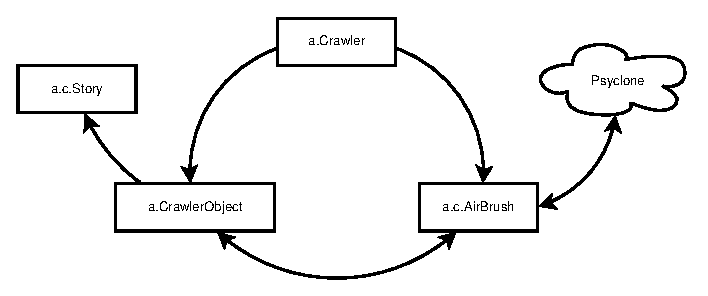
\includegraphics{image/crawler}
  \caption{
    Diagram of the design of the Crawler, the names are Java classnames
  }
\end{figure}



\section{Objects in the amber.sieve package}



\classname{KeywordSpotter}

\begin{classmetadata}
  \extends{SieveObject}
  \implements{amber.common.AirBrushCallable}
  \function{The KeywordSpotter is configured to detect the presence of certain
            keywords in a story which makes it fit in a certain category or
            subject. In early versions the weights of the subjects will be
            equal. In later versions all weights of all subjects of a story
            must for instance add up to 100\%.  This gives the visualizer more
            freedom to place the story.}
\end{classmetadata}

% \begin{interface}
% \end{interface}



\classname{PhraseSpotter}

\begin{classmetadata}
  \extends{SieveObject}
  \implements{amber.common.AirBrushCallable}
  \function{The PhraseSpotter will use a grammar engine to detect whether
            certain types of sentences appear in a story to classify it.}
\end{classmetadata}

% \begin{interface}
% \end{interface}



\subsection{Objects in the amber.showoff package}


\begin{figure}[htp]
  \centering
  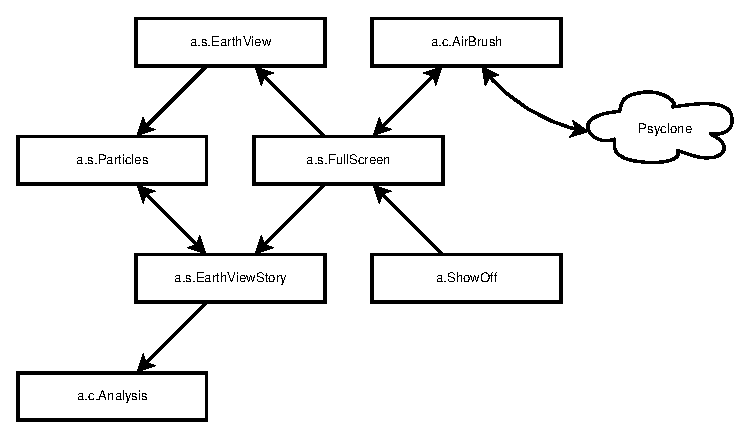
\includegraphics{image/showoff-fullscreen}
  \caption{\label{fig:showoff-fullscreen}Object model of the full screen
    ShowOff module. Arrows represent the presence of references to the object
    where it is pointing to in the object where it is pointing from. The object
    model of the applet is about equal to this one.}
\end{figure}


\classname{Applet}

\begin{classmetadata}
  \extends{amber.ShowOff}
\end{classmetadata}

% \begin{interface}
% \end{interface}


\classname{Attractor}

\begin{classmetadata}
\end{classmetadata}

% \begin{interface}
% \end{interface}


\classname{EarthView}

\begin{classmetadata}
  \extends{javax.swing.JPanel}
  \implements{Runnable}
  \dependencies{FullScreen, StoryLauncher}
  \function{EarthView is a graphical user interface element based on a JPanel
      which displays a picture of Earth in space, with particles orbiting
      around it. Attractors can be added to influence the orbits of the
      particles.}
  \processing{There is a list of particles, which contains information on
      their location and more. EarthView draws each of the particles in the
      list on itself.}
\end{classmetadata}

\begin{interface}
  \init{EarthView}{\mbox{Collection$\langle$Particle$\rangle$} pc}
    {Initializes the EarthView display. It is a child of JPanel and can as such
    be used inside any Swing application. Before starting the Earthview, first
    couple a Particle collection to it using setParticleCollection.}
    \method{\void}{setParticleCollection}{\mbox{Collection$\langle$Particle$\rangle$} pc}
    {Sets the collection of particles to be displayed in the view.}
  \method{\void}{run}{}
    {Runs the thread (for Runnable).}
  \method{\void}{start}{}
    {Starts the thread, lets EarthView draw stuff.}
\end{interface}


\classname{EarthViewStory}


\classname{FullScreen}

\begin{classmetadata}
  \extends{amber.ShowOff}
  \implements{amber.common.AirBrushCallable}
  \dependencies{ShowOff}
  \function{This is a ShowOff module which displays the visualization in full
    screen size.}
\end{classmetadata}

\begin{interface}
  \init{FullScreen}{}
    {Initializes something.}
  \method{\void}{start}{}
    {Start the visualization.}
  \method{void}{airBrushReceiveMessage}{Message msg}
    {}
\end{interface}


\classname{ObservableList}


\classname{Particle}

\begin{classmetadata}
  \function{Storage of particle data.}
  \data{An object of this class has information about its location and
    velocity, and it knows from which story it originates.}
  \dependencies{StoryLauncher, Particles}
\end{classmetadata}

\begin{interface}
  \init{Particle}{Story s}
    {Initializes a particle for Story s.}
  \method{\void}{launch}{}
    {Launches the particle, all parameters must be set, they cannot be changed
      afterwards.}
  \method{\void}{boost}{double}
    {Boost the particle in the direction it is heading. This can happen when
      for instance the Story gets replies or comments; boosting keeps the
      particle around longer.}
  \method{double}{getMass}{}
    {Gets the mass of the particle}
  \method{Point2d}{getLocation}{}
    {Gets the location}
  \method{Vector2d}{getVelocity}{}
    {Gets the velocity}
  \method{Vector2d}{getAcceleration}{}
    {Gets the acceleration}
  \method{\void}{calculate}{double t}
    {Calculates and sets new values using the current values after a period of
      time t}
\end{interface}

The Particles' location is represented by polar coordinates, with ``earth''
being the origin (0, 0).

A particle can be in one of five states: new, launch, orbit, boost or crashed.
Every particle will obviously start in the ``new'' state, after which it is
launched and gets into ``launch'' state. In this state, the $r$ component will
grow until it reaches a set height above the surface of earth, while $\theta$
also accellerates to a set speed. When these values are reached, the particle
will be in orbit and thus in state ``orbit''.

In orbit, a particle slows down and slowly falls back to the earth until it
reaches some lower bound when it is considered ``crashed''. While a particle is
in orbit, it can get a speed increase, it will get in ``boost'' state. During
this period, the height and speed are increased, hereby keeping the particle
orbiting earth for a prolonged time.

While in orbit, a particle can also be attracted by certain attractors that are
located outside the orbits, dependent on the topic of the story it represents.



